\chapter{Entrenar}
\label{cap:entrenar}

\begin{enpocas}
El optimizador MuSGD, la tasa de aprendizaje con calentamiento, el promedio móvil
de pesos (EMA) y el ciclo que junta todo. Al final, el comando para entrenar
FuegoNet-n desde cero y lo que pasó en las 150 épocas. Archivos:
\cod{red_fuego/optimizador.py} y \cod{red_fuego/entrenar.py}.
\end{enpocas}

\section{El optimizador MuSGD}

Entrenar es repetir: calcular la pérdida de un lote, obtener el gradiente
$\mathbf{g} = \nabla L$ con \cod{backward()} y mover los pesos un poco en
contra. El descenso por gradiente estocástico con momento (SGD) hace
\begin{equation}
\mathbf{m} \leftarrow \mu\,\mathbf{m} + \mathbf{g},\qquad
\mathbf{W} \leftarrow \mathbf{W} - \eta\,(\mathbf{g} + \mu\,\mathbf{m})\quad\text{(Nesterov)}.
\end{equation}

\textbf{Muon} trata cada matriz de pesos como un todo. Una convolución
$c_{\text{out}}\times c_{\text{in}}\times k\times k$ se ve como matriz
$\mathbf{G}$ de $c_{\text{out}}\times(c_{\text{in}}k^2)$. Si
$\mathbf{G} = \mathbf{U}\mathbf{S}\mathbf{V}^\top$ (descomposición en valores
singulares), Muon cambia la actualización por $\mathbf{U}\mathbf{V}^\top$: la
misma dirección, pero con \emph{todos} los valores singulares iguales a 1. Ninguna
dirección domina a las demás y las «débiles» también avanzan.

Calcular la SVD en cada paso sería lentísimo. Muon aproxima
$\mathbf{U}\mathbf{V}^\top$ con cinco iteraciones de Newton-Schulz, solo con
multiplicaciones de matrices:
\begin{equation}
\mathbf{X}_0 = \frac{\mathbf{G}}{\|\mathbf{G}\|_F},\qquad
\mathbf{A} = \mathbf{X}\mathbf{X}^\top,\qquad
\mathbf{X} \leftarrow a\,\mathbf{X} + (b\,\mathbf{A} + c\,\mathbf{A}^2)\,\mathbf{X},
\end{equation}
con $a = 3.4445$, $b = -4.7750$ y $c = 2.0315$.

\paso{19} \textbf{Escribir \cod{ortogonalizar} y \cod{MuSGD}.}
\begin{lstlisting}[style=py]
def ortogonalizar(G, pasos=5, eps=1e-7):
    a, b, c = 3.4445, -4.7750, 2.0315
    X = G.bfloat16()
    X = X / (X.norm() + eps)                 # valor singular mayor <= 1
    alta = G.size(0) > G.size(1)
    if alta:
        X = X.T
    for _ in range(pasos):
        A = X @ X.T
        X = a * X + (b * A + c * A @ A) @ X
    return (X.T if alta else X).to(G.dtype)
\end{lstlisting}

YOLO26 aplica a los pesos de convolución las \emph{dos} actualizaciones, Muon con
factor 0.2 y SGD con factor 1:
\begin{equation}
\mathbf{W} \leftarrow \mathbf{W} - 0.2\,\eta\,\mathrm{Muon}(\mathbf{g})
\sqrt{\max(1, c_{\text{out}}/c_{\text{in}}k^2)}
- \eta\,\mathrm{SGD}(\mathbf{g} + \lambda\mathbf{W}),
\end{equation}
y a los sesgos y a BatchNorm solo SGD, sin decaimiento de pesos ($\lambda = 0$).

\section{Tasa de aprendizaje, calentamiento y lote nominal}

\begin{itemize}
  \item \textbf{Ley lineal}: $\eta(e) = \eta_0\,[(1 - e/E)(1 - 0.01) + 0.01]$, de
        $\eta_0 = 0.01$ a $0.0001$.
  \item \textbf{Calentamiento}: en las primeras 3 épocas $\eta$ sube desde 0 (los
        sesgos bajan desde 0.1) y el momento de 0.8 a 0.9. Con pesos al azar, un paso
        grande al principio puede arruinar las estadísticas de BatchNorm.
  \item \textbf{Lote nominal 64}: con lotes de 32 se acumulan dos gradientes antes de
        cada paso. El decaimiento de pesos se escala por $32\cdot2/64 = 1$.
  \item \textbf{Recorte}: la norma del gradiente se limita a 10.
\end{itemize}

\section{EMA: el modelo suavizado}

Se guarda una copia de la red cuyos pesos son un promedio móvil exponencial de
los pesos de entrenamiento:
\begin{equation}
\mathbf{W}_{\text{EMA}} \leftarrow d\,\mathbf{W}_{\text{EMA}} + (1-d)\,\mathbf{W},\qquad
d = 0.9999\,\big(1 - e^{-n/2000}\big),
\end{equation}
donde $n$ es el número de pasos dados. La EMA ignora el «temblor» de cada lote. Es
la que se valida y se guarda.

\section{El ciclo de entrenamiento}

\paso{20} \textbf{Escribir el ciclo.}
Lo esencial de \cod{entrenar.py}:
\begin{lstlisting}[style=py]
for epoca in range(a.epocas):
    perdida.fijar_epoca(epoca)                     # ProgLoss
    for k, lote in enumerate(carga_ent):
        ...                                        # calentamiento de lr y momento
        lote['img'] = lote['img'].to(disp).float() / 255
        with torch.autocast('cuda', torch.bfloat16):
            pred = modelo(lote['img'])             # {'o2m': ..., 'o2o': ...}
        l, partes = perdida(pred, lote)
        (l / acumular).backward()
        if (k + 1) % acumular == 0:
            torch.nn.utils.clip_grad_norm_(modelo.parameters(), 10.0)
            opt.step(); opt.zero_grad(set_to_none=True)
            ema.actualizar(modelo)
    m = validar(ema.m, carga_val, nc, disp)        # mAP en las 600 de validación
    # guarda ultimo.pt y, si 0.1 mAP50 + 0.9 mAP50-95 mejoró, mejor.pt
\end{lstlisting}

\begin{nota}
\cod{torch.autocast} con \cod{bfloat16} hace las convoluciones en 16 bits (más
rápido, la mitad de memoria) y deja en 32 bits lo delicado. A diferencia de
\cod{float16}, \cod{bfloat16} tiene el mismo rango que \cod{float32}, así que no
necesita \cod{GradScaler}. Las tarjetas RTX de la serie 30 en adelante lo
soportan.
\end{nota}

\paso{21} \textbf{Primera prueba: tres épocas.}
Antes de lanzar horas de entrenamiento se corre una prueba corta. Si hay un error
en la asignación o en la pérdida, el mAP se queda en cero:
\begin{lstlisting}[style=bash]
~/.venvs/yolo/bin/python -m cuadrirotor_sim.red_fuego.entrenar \
  --datos ~/datasets/combinado_incendio_bosque_incendio_bosque_grande/data.yaml \
  --epocas 3 --salida /tmp/prueba_fuegonet
\end{lstlisting}
\begin{resultado}
\begin{lstlisting}
FuegoNet-n: 2.50 M parámetros, 5400 imágenes de entrenamiento, 600 de validación
[  1/3] pérdida caja 3.364 clase 8.700 dist 0.045 | mAP50 0.001 mAP50-95 0.000 | 74 s
[  2/3] pérdida caja 3.004 clase 4.437 dist 0.042 | mAP50 0.077 mAP50-95 0.022 | 122 s
[  3/3] pérdida caja 2.507 clase 2.656 dist 0.034 | mAP50 0.512 mAP50-95 0.198 | 171 s
\end{lstlisting}
Las tres pérdidas bajan y el mAP50 sube de 0 a 0.5 en tres épocas, sin ningún
peso preentrenado. La red está aprendiendo.
\end{resultado}

\paso{22} \textbf{Entrenamiento completo.}
\begin{lstlisting}[style=bash]
nohup ~/.venvs/yolo/bin/python -m cuadrirotor_sim.red_fuego.entrenar \
  --datos ~/datasets/combinado_incendio_bosque_incendio_bosque_grande/data.yaml \
  --epocas 150 --salida ~/datasets/fuegonet/n_150 > ~/datasets/fuegonet/n_150.log 2>&1 &
tail -f ~/datasets/fuegonet/n_150.log
\end{lstlisting}
Cada época queda en una fila de \cod{resultados.csv}: tiempo, las tres pérdidas
de la o2o, P, R, mAP50, mAP50-95, AP por clase, tasa de aprendizaje y peso $w$
de ProgLoss.

\section{Qué pasó en el entrenamiento}

\begin{figure}[H]
\centering
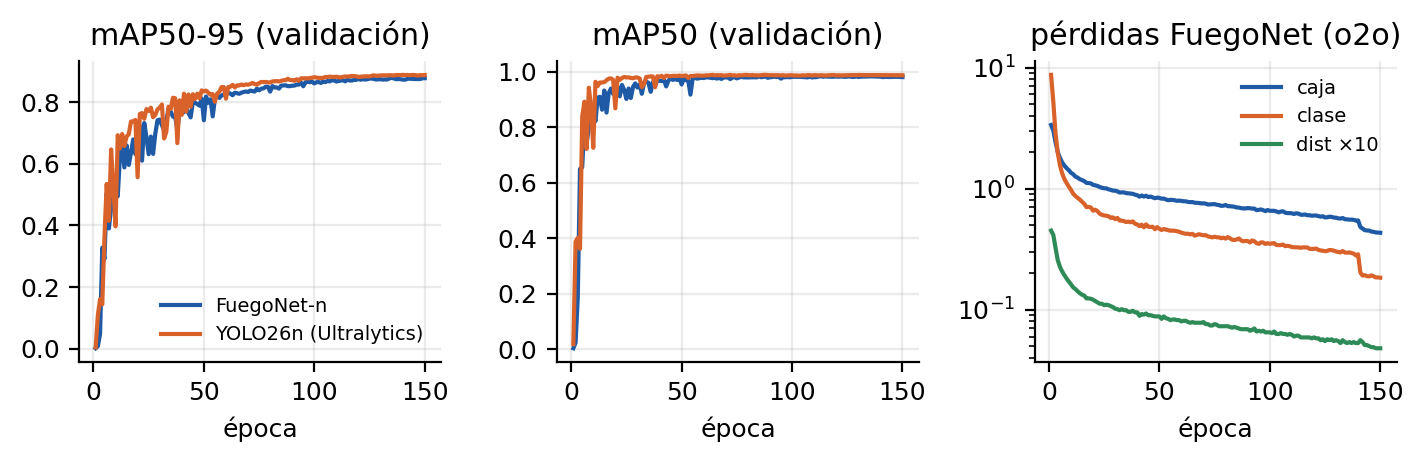
\includegraphics[width=\textwidth]{curvas.png}
\caption{Entrenamiento desde cero. Izquierda y centro: mAP en validación de
FuegoNet-n (este manual) y de YOLO26n de Ultralytics con la misma receta.
Derecha: pérdidas de la cabeza o2o de FuegoNet (escala logarítmica).}
\label{fig:curvas}
\end{figure}

\begin{itemize}
  \item El entrenamiento corrió 150 épocas en 156 minutos
        (unos 62~s por época, compartiendo la
        GPU con la corrida de control).
  \item El mejor modelo (\cod{mejor.pt}) es el de la época 135: mAP50 =
        0.984 y mAP50-95 = 0.879 en validación
        (AP50-95 de fuego 0.879, de humo 0.879).
  \item En la época 10 ya tenía mAP50 = 0.859: la mayor parte se aprende
        pronto y las últimas épocas afinan las cajas (sube sobre todo el mAP50-95).
  \item Al apagar el mosaico (últimas 10 épocas) hay un salto pequeño hacia arriba: la
        red se ajusta a imágenes completas como las de vuelo.
\end{itemize}

\begin{nota}
La curva naranja es el control: YOLO26n de Ultralytics, también desde cero, con los
mismos datos y aumentos. Su mejor época (140) da mAP50-95 =
0.889 \emph{según su propio validador}. La comparación
justa, con el mismo código de métricas, está en el capítulo~\ref{cap:evaluar}.
\end{nota}

